\subsection{Individual Project Report for Alexandra Kapp}
\par \underline{ECTS:} 6
\par \underline{Hours spent so far:} 147 
\par \underline{Short description of the tasks done so far:}
\begin{itemize}
\item Familiarize myself the work of the Beacon group. Get to know what has been done so far, how the technology works and what is to come.
\item Make improvements on the questionnaire and discuss the translation into German.
\item Work on the simulation:
\begin{itemize} 
\item Main question to answer: How many beacons can be detected under different circumstances in the future?
\item Implement a simulation setting of the ERBA building with different rooms, entrances, cafeteria and library.
\item Identify variables of interest for the simulation: E.g. Android share vs. iPhone share in Germany, percentage of devices which are suitable for beacon detection, people with Bluetooth turned on, etc.
\item Get data:
\begin{itemize} 
\item Find literature and studies on the identified factors that relate to beacon detections
\item Find reasonable future values on those parameters (e.g. share of Android phones with an os > 
\end{itemize}
Android 5.0 will likely rise from 70% to 95% within the next 3-5 years)
\item Replicate the results that we found with our deployed beacons in the simulation.
\item Change parameters to reasonable future values and create a future average case scenario
\item Imagine the best values that are still somewhat possible for the factors. Simulate a best-case scenario for the future.
\item Write the simulation part of the report and make the respective presentation part. 
\end{itemize}
\end{itemize}

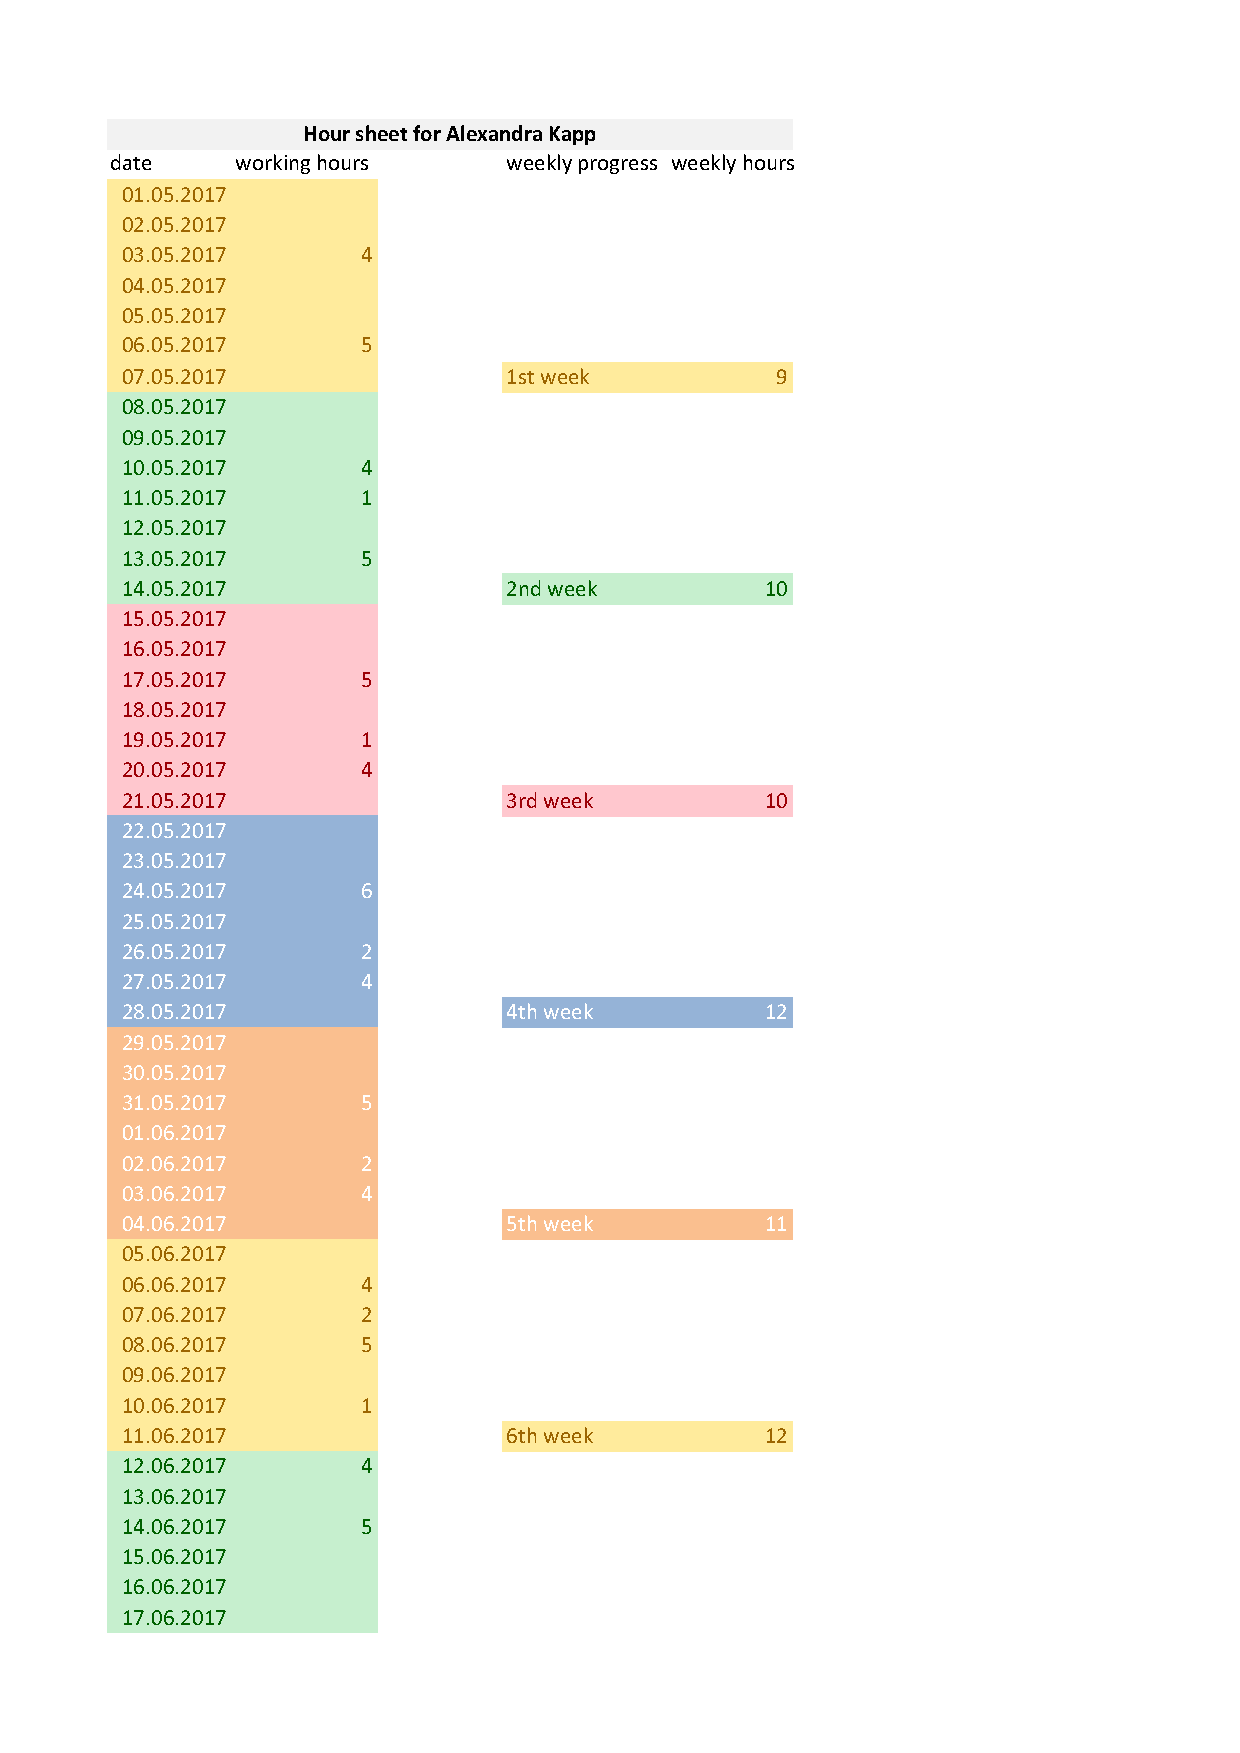
\includepdf[pages={-}]{appendix/studentHoursTemplate_AlexandraKapp.pdf}

